\documentclass{article}
% Camera-ready: the official style with the workshop track plus [final]; the style
% file is byte-identical to the official NeurIPS 2026 template.
\usepackage[dblblindworkshop,final,nonatbib]{neurips_2026}
\workshoptitle{SLMs for Agentic Systems, Paris, France, 2026}  % as required by the OpenReview camera-ready form

\usepackage[utf8]{inputenc}
\usepackage[T1]{fontenc}
\renewcommand{\ttdefault}{lmtt}  % Type 1 typewriter; EC tt would embed as Type 3 bitmaps
\usepackage[hidelinks]{hyperref}
\hypersetup{pdftitle={Can a Knowledge-Graph Agent Close the Gap Between a Low-Cost and a Frontier-Class LLM? An Audited Upstream Petroleum Case Study}, pdfauthor={Tousifahamed Allabksha Nadaf}}
\usepackage{url}
\usepackage{booktabs}
\usepackage{array}
\usepackage{longtable}
\usepackage{amsfonts}
\usepackage{amssymb}
\usepackage{nicefrac}
\usepackage{microtype}
\usepackage{xcolor}
\usepackage{graphicx}
\usepackage{amsmath}

\title{Can a Knowledge-Graph Agent Close the Gap Between a Low-Cost and a
Frontier-Class LLM? An Audited Upstream Petroleum Case Study}

\author{
  Tousifahamed Allabksha Nadaf \\
  Wipro \\
  \texttt{tousifahamed.nadaf@wipro.com}, \texttt{ahamedpapers@gmail.com}\thanks{Corresponding email address.}
}

\begin{document}

\maketitle

\begin{abstract}
Small, low-cost language models are attractive agent backbones but are assumed
to trail frontier models on tasks requiring exact identifiers, deterministic
aggregation, and multi-hop reasoning. We test how close a knowledge-graph (KG)
agent brings them. One ReAct pipeline -- a structured graph-query tool, a
deterministic aggregation tool, and a citation-traceability guardrail
-- runs a 50-question upstream-petroleum benchmark with a low-cost backbone
(Gemini~3.1~Flash-Lite) and a frontier-class one (Claude~Opus~4.8), three
repeats each. Normalized exact match (EM) gives \textbf{0.898} vs.\
\textbf{0.889}; a symmetric hand audit of all 216 EM answers gives
\textbf{0.926} vs.\ \textbf{0.954}, and the backbones differ on only 3 of 36
items, so this benchmark cannot separate them. The audit also shows that most
strict-EM failures of both backbones are correct answers (82\% and 81\%), that
grading rules derived from one backbone missed a format of the other, and that
7 of the 50 items are defective. An ablation ladder places the gain in the
graph plus deterministic tools: graph retrieval without agency scores
\textbf{0.278}, below Text-RAG at \textbf{0.583}. Since gold answers are
computed from the graph the tools query, we read this as both backbones driving
one toolchain to similar accuracy, not as a claim about model size.
\end{abstract}

\section{Introduction}

Small language models (SLMs) are attractive as agent backbones: cheaper,
faster, and often free-tier-accessible, which matters for who can afford to
deploy agentic tools at all. The standard assumption is that this comes at a
capability cost on tasks needing exact identifiers, deterministic
aggregation, and multi-hop reasoning -- exactly the profile of upstream
petroleum analytics, where analysts mix identification (\emph{which well}),
risk assessment (\emph{is this pair a breakthrough risk}), recommendation
(\emph{what is the cheapest fix}), and causal explanation (\emph{why}) over
well topology, injector-producer connectivity, time-series sensor readings,
alerts, and recommended interventions. We ask how much of that capability cost
a better-structured pipeline can remove, rather than a bigger model.

Standard text-based RAG treats this domain as unstructured passages: it can
retrieve topically relevant text, but it cannot compute rankings or
aggregates, and it is prone to inventing plausible-looking but fake
identifiers (e.g., intervention IDs) when asked to rank or recommend.
Knowledge-graph RAG
(KG-RAG)~\cite{lewis2020rag,edge2024graphrag,sanmartin2024kgrag,pan2024roadmap}
promises structure-aware retrieval and agentic tool
use~\cite{yao2023react,schick2023toolformer} promises deterministic
computation, but whether combining both lets a low-cost backbone do as well as
a frontier one, and how such a system behaves when the graph is incomplete or
noisy, remains relatively underexplored.

We present a knowledge-graph agent that combines (1) a structured graph-query
tool, (2) a deterministic aggregation tool, and (3) a citation guardrail that
rejects identifiers no tool returned, and evaluate it under two API backbones
and against text-RAG and graph-retrieval-only baselines on a 50-question
benchmark built from the public Volve field dataset, used here as a demanding
testbed rather than as the paper's primary claim. We study two research
questions. \textbf{RQ1 (backbone dependence):} with the same KG agent, how close
do a low-cost and a frontier-class backbone come, and which parts of the
scaffold account for the result? \textbf{RQ2 (robustness, preliminary):} how
does the agent's accuracy change when the graph is incomplete or its
connectivity weights are noisy? Our contributions are:

\begin{enumerate}
  \item A cross-backbone comparison with a symmetric audit (RQ1): under one
  pipeline the two backbones come within one EM item per repeat of each other
  (audited EM 0.926 vs.\ 0.954), a difference this 36-item benchmark cannot
  resolve; we report similar accuracy, not parity
  (Section~\ref{sec:results}).
  \item An instance-level audit of both backbones' answers (RQ1) that separates
  model errors from grader artifacts and benchmark defects: most strict-EM
  failures of both backbones are correct answers, a normalized grader built from
  one backbone's failures missed a format of the other, and seven benchmark
  items are defective.
  \item An ablation ladder (RQ1) in which graph structure alone scores
  \emph{lower} than text retrieval and the deterministic aggregation tool
  accounts for the largest single share of the full agent's score.
  \item A preliminary robustness probe (RQ2) on the low-cost backbone, with the
  perturbations, and the evidence they can and cannot reach, stated exactly.
\end{enumerate}
Code, data, run logs, and audit verdicts are available at
\url{https://github.com/TousifAhamed/kg-agent-low-cost-vs-frontier}.

\section{Related Work}

\textbf{KG-RAG and graph-structured retrieval.} GraphRAG~\cite{edge2024graphrag}
and related work~\cite{sanmartin2024kgrag} summarize community structure in a
knowledge graph to answer global, corpus-level questions; Think-on-Graph~\cite{sun2024tog}
performs beam search over KG relations, showing that a strong graph can let a
smaller LLM match a larger one, a hypothesis we test in a new domain.
Pan et al.~\cite{pan2024roadmap} survey the broader space of unifying LLMs and
KGs. We build on classical RAG~\cite{lewis2020rag} (see Gao
et al.~\cite{ragsurvey2023} for a survey of the RAG design space) but replace
passage retrieval with structured graph queries plus deterministic tools.

\textbf{Agentic tool use.} Chain-of-thought prompting~\cite{cot2022}
established that intermediate reasoning traces improve LLM task performance;
ReAct~\cite{yao2023react} interleaves such traces with tool actions, and
Toolformer~\cite{schick2023toolformer} teaches models to invoke APIs. Qin et
al.~\cite{toollearning2023} and Wang et al.~\cite{llmagents2024} survey the
broader tool-use and autonomous-agent literature. Our agent follows the ReAct
pattern but adds a domain-specific deterministic aggregation tool and a
post-hoc citation guardrail, rather than relying on the LLM to compute
rankings itself.

\textbf{Ontologies and hallucination.} We anchor entities to a minimal subset
of the ISO 15926 process-industry data model~\cite{iso15926}, maintained by the
POSC~Caesar Association, within a knowledge graph~\cite{hogan2021kgsurvey} that
carries a W3C PROV-O provenance profile~\cite{provo2013}, so every tool result
carries a traceable node id. Ji et al.~\cite{ji2023hallucination} survey
hallucination in NLG; our citation guardrail is a lightweight, verifiable
traceability check in the spirit of self-verification approaches such as
Self-RAG~\cite{selfrag2024}.

\textbf{Domain analytics.} Capacitance-resistance modeling
(CRM)~\cite{yousef2006crm,sayarpour2009} and Chan's water-cut/WOR diagnostic
plots~\cite{chan1995wor} are standard reservoir-engineering tools for inferring
injector-producer connectivity and diagnosing coning/channeling; we encode
their outputs as first-class KG edges and node properties rather than leaving
them to unstructured retrieval.

\section{Method}

\textbf{Knowledge graph.} We build a property graph~\cite{graphdb2008} over production and injection records from the public
Volve field dataset (5 producers, 2 injectors, 2007--2016). Alerts,
interventions, and derived diagnostic edges are not in the raw field release;
they are generated once from the real series by fixed rules (first water cut
$\geq 0.50$ $\to$ breakthrough alert, water cut $\geq 0.90$ $\to$ severe alert,
$\log_{10}\mathrm{WOR} \geq 0$ $\to$ high-WOR alert, one recommended
intervention with sampled cost and uplift per breakthrough or severe alert;
Appendix~\ref{app:benchmark}). This single instantiation is the KG seed for all
experiments. The graph has 7 node types (\texttt{Well}, \texttt{Reservoir},
\texttt{Sensor}, \texttt{MetricReading}, \texttt{Alert},
\texttt{Intervention}, \texttt{Field}) and 6 relation types, each carrying a
PROV \texttt{wasDerivedFrom} edge~\cite{provo2013} (provenance coverage 1.0).
All reported runs query an in-memory NetworkX copy of the graph; a Cypher export
for Neo4j 5.26 exists but was not queried in these experiments.

\textbf{Agent.} An entity linker~\cite{entitylink2015} seeds the first turn
with mentioned KG node ids; a ReAct loop (max 5 tool rounds) then selects among
\texttt{cypher\_query} (despite its name, a structured tool: the model picks
an operation -- label/filter search, neighbours, $k$-hop subgraph, latest
reading -- and filters, rather than writing Cypher), \texttt{compute\_metric} (deterministic count / sum / mean /
min / max / rank, including derived ratios such as cost-per-barrel), and
\texttt{semantic\_search} (FAISS~1.9.0~\cite{faiss2017} over the
serialized-dashboard corpus of the Text-RAG baseline, as a fuzzy fallback). A
citation guardrail checks \emph{traceability}, not support: it accepts a cited
id only if the id exists in the graph and was returned by a tool during that
run (retrying up to twice), so it blocks fabricated identifiers but does not
verify that a cited node supports the claim made about it. The low-cost
backbone is \texttt{gemini-3.1-flash-lite}~\cite{gemini31flashlite}, accessed
through the Gemini API free tier; it is Google's most cost-efficient Gemini
3-series model and its parameter count is not published, so we call it
``small'' and ``low-cost'' in the sense of price tier only. The large backbone is
\texttt{claude-opus-4-8}~\cite{claudeopus48}, a frontier-class commercial model
at the time of the study. Both use the provider's default decoding temperature
and a 1024-token output cap, and the full agent was run three independent
times on each. Large-backbone runs were made on 2026-07-03 and small-backbone
runs on 2026-07-17--22, through floating API aliases without logged snapshot
identifiers; the two-week gap is a confound we cannot remove, and exact
re-execution against the same weights is not guaranteed.

\textbf{Baselines.} \emph{S1 (LLM-only)}: no retrieval or tools. \emph{S2
(Text-RAG)}: FAISS dense retrieval~\cite{dpr2020} ($k{=}10$) over serialized
dashboard documents with the \texttt{all-MiniLM-L6-v2}
Sentence-BERT~\cite{sbert2019} embedder (sentence-transformers 3.3.1).
\emph{S3 (KG-retrieval-only)}: $k$-hop subgraph serialization into a single
LLM call, with no tools and no agent loop.

\section{Experimental Setup}

\textbf{Benchmark.} 50 questions (13 Identification, 12 Risk, 13
Recommendation, 12 Explanation), instantiated from templates by a script that
computes each gold answer by traversal or aggregation over the KG;
Appendix~\ref{app:benchmark} lists all 50. The templates were drafted before
any agent code existed, but were instantiated against the KG in the same week
the agent's tools were built, so tool design was not blind to the question
set. We report EM over the 36 string- or number-answerable items, NDCG@5~\cite{ndcg2002}
over the 2 ranking items, citation validity, and a 0--3 rubric over the 12
Explanation items, scored by an LLM judge~\cite{llmjudge2023} given the gold
evidence nodes; the judge is the backbone being scored, so rubric scores are
not comparable across backbones (Appendix~\ref{app:explanation}).

\textbf{Grading.} Strict EM applies a 2\% numeric tolerance and ordered
number matching for multi-number answers. Normalized EM additionally scans
every number in a prose answer (strict takes only the first, which can pick
the ``5'' out of ``\texttt{F-5}''), normalizes prose dates, squashes
underscores and hyphens, and discounts well ids echoed from the question
(Appendix~\ref{app:grading}). These four rules were written \emph{after}
auditing the small backbone's failures, so they are tuned on one arm of the
comparison, and a check that S1--S3 are unchanged by them cannot detect a rule
that favors prose. We therefore also audit every EM answer of both backbones by
hand against the question as worded (Section~\ref{sec:results},
Appendix~\ref{app:audit}).

\textbf{Repeats and perturbations.} The full agent runs three times per
backbone; the two ablations and the four perturbation conditions run once, on
the small backbone only. Edge dropout at rate $p$ removes each
\texttt{INJECTS\_INTO} edge and each \texttt{MetricReading} node independently
with probability $p$; weight noise at relative $\sigma$ multiplies each
\texttt{INJECTS\_INTO} connectivity weight by $1+\epsilon$,
$\epsilon \sim \mathcal{N}(0,\sigma^2)$, clipped at 0. Each condition is a
single draw (seed 42), with gold answers fixed to the clean graph. Neither
perturbation touches alert, intervention, or well nodes, and the
\texttt{semantic\_search} fallback indexes the unperturbed corpus.

\section{Results}
\label{sec:results}

\begin{table}[t]
  \centering
  \small
  \caption{Full agent, 36 EM items, 3 repeats per backbone (108 answers each).
  ``Audited'' judges every answer by hand against the question as worded, with
  corrected gold for defective items (Appendix~\ref{app:audit}).}
  \label{tab:audit}
  \begin{tabular}{lcc}
    \toprule
    & Small (Flash-Lite) & Large (Opus 4.8) \\
    \midrule
    Strict EM & 0.741 & 0.852 \\
    Normalized EM (repeats 1/2/3) & 0.898 (.917/.861/.917) & 0.889 (.889/.889/.889) \\
    Audited EM (repeats 1/2/3) & 0.926 (.944/.889/.944) & 0.954 (.972/.944/.944) \\
    \midrule
    Strict-EM failures & 28 & 16 \\
    \quad artifact, fixed by normalization & 17 & 4 \\
    \quad artifact, missed by normalization & 0 & 2 \\
    \quad defective item, correct as worded & 6 & 7 \\
    \quad genuine error & 5 & 3 \\
    Normalized credit, wrong on audit & 3 & 2 \\
    \bottomrule
  \end{tabular}
\end{table}

\textbf{Similar accuracy, not parity (RQ1, Table~\ref{tab:audit}).} Under
normalized EM the small backbone scores 0.898 and the large 0.889. But
normalization lifts the small backbone by 15.7 points and the large by 3.7,
and its rules came from the small backbone's failures, so we audited all 216
EM answers of both. Every answer the normalized grader newly accepts is
correct for both backbones, so we found no credit for incidentally mentioned
numbers; but the rules miss a format only the large backbone uses (``5/5 =
100\%''), and the audit exposed two defective EM items: Q19's gold value comes
from a generator bug (the correct answer is ``yes''), and Q25 asks how many
producers ``currently'' exceed 90\% water cut (one) while its gold counts those
that ever did (two). On audit the scores are 0.926 (small) and 0.954 (large).
The backbones' item-level means differ on 3 of the 36 items, all in the large
backbone's favor (two-sided sign test $p=0.25$; paired item bootstrap 95\% CI
for small minus large $[-0.065, 0.000]$; under normalized EM $[-0.019,
+0.046]$). The benchmark therefore cannot separate the two backbones, and the
audited point estimate favors the large one by one item per repeat. S2 and S3
score identically for both backbones (0.583 and 0.278); S1 scores 0.028 (small)
and 0.056 (large), the extra credit being a non-answer to the defective Q19
that the boolean grader counts as ``no''. Because the backbones also tie
without the agent, these results show both reaching similar accuracy through
the pipeline, not the pipeline closing a gap measured here.

\textbf{What the scaffold contributes (RQ1).} The ablations
(Figure~\ref{fig:main}, small backbone) show graph structure alone is not
enough: S3 (0.278) scores below S2 (0.583), since a serialized raw subgraph is
a weaker signal than ranked dense passages for this question set. Removing
\texttt{compute\_metric} drops normalized EM from 0.898 to 0.750 (strict 0.667)
and NDCG@5 from 1.000 to 0.659 -- the agent still \emph{finds} the right
entities but can no longer \emph{rank} them. Removing the guardrail costs less
EM (0.861) and lowers citation validity from 1.00 to 0.98. These effects are
partly built into the benchmark: gold answers to aggregation items are, by
construction, what \texttt{compute\_metric} returns over the same graph, and
S1 scoring 1--2 of 36 shows the items are unanswerable without the tools. The
ablation therefore says which tools this toolchain needs, not how graph and
text retrieval compare in general. Rubric scores and NDCG@5 are in
Appendix~\ref{app:explanation}.

\begin{figure}[t]
  \centering
  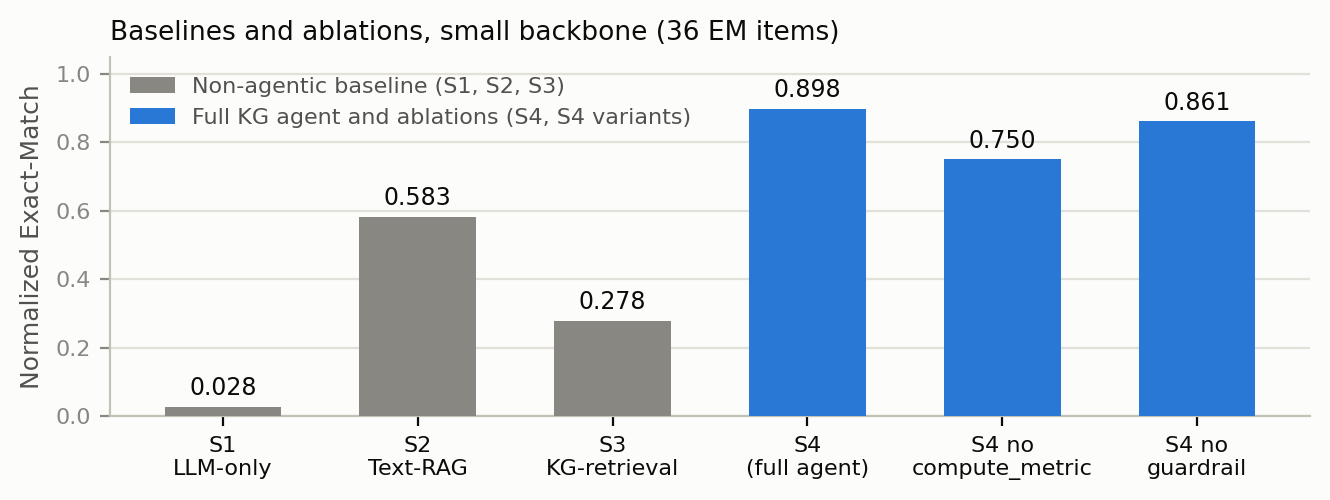
\includegraphics[width=0.85\textwidth]{figures/fig_main_results.png}
  \caption{Normalized EM on the 36 EM items, small backbone. S4 is a 3-repeat
  mean; the two S4 ablations and the baselines are single runs. S2 and S3 score
  the same with the large backbone; S1 scores 0.056 there.}
  \label{fig:main}
\end{figure}

\begin{figure}[t]
  \centering
  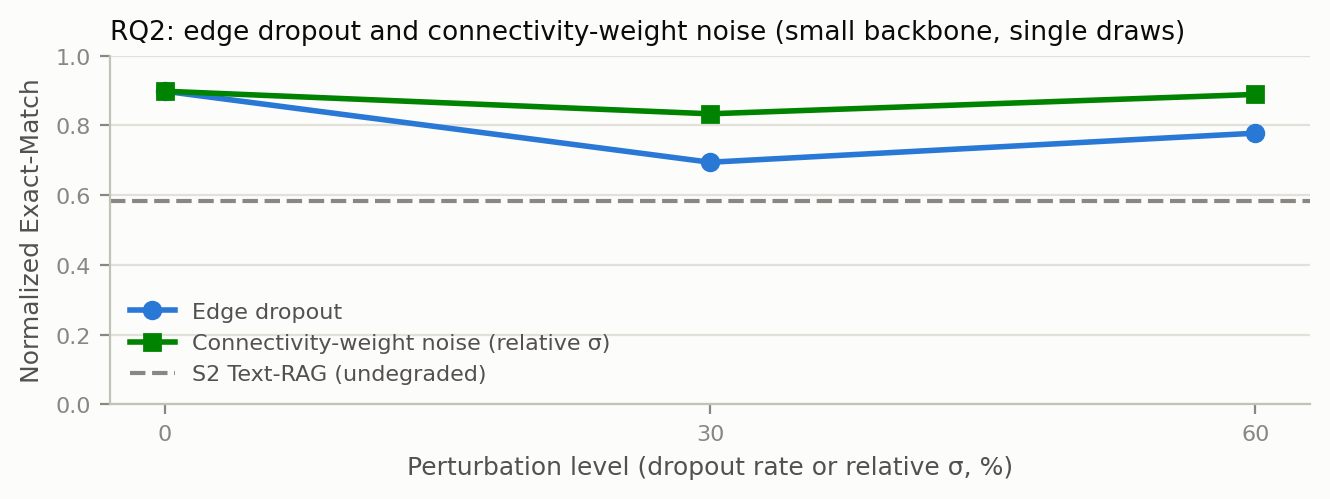
\includegraphics[width=0.85\textwidth]{figures/fig_robustness.png}
  \caption{Normalized EM under edge dropout and connectivity-weight noise,
  small backbone, gold fixed to the clean graph. Each perturbed point is one
  draw; the 0\% point is the 3-repeat mean. Dashed line: undegraded Text-RAG.}
  \label{fig:robustness}
\end{figure}

\textbf{Robustness, preliminary (RQ2, Figure~\ref{fig:robustness}).}
Normalized EM at 0 / 30 / 60\% edge dropout is 0.898 / 0.694 / 0.778, and at
relative weight noise $\sigma$ = 0 / 0.3 / 0.6 it is 0.898 / 0.833 / 0.889; all
four perturbed scores stay above the undegraded Text-RAG baseline (0.583).
These numbers are weaker evidence than they look. Of the 36 EM items, 20 rest
only on alert, intervention, or well properties that neither perturbation
alters, weight noise reaches the evidence of only 8, and the fallback search
can still return clean values. On those 8 weight items, noise lowers EM from
0.833 to 0.625 ($\sigma$=0.3) and 0.750 ($\sigma$=0.6), while untouched items
barely move; under 30\% dropout, both touched (0.854 $\to$ 0.625) and untouched
(0.933 $\to$ 0.750) items fall, which single draws cannot attribute to the
perturbation rather than run-to-run variation. Neither curve is monotonic, and
with one backbone the probe does not test whether similar accuracy holds under
corruption.

\section{Limitations and Future Work}
\label{sec:limits}

\textbf{Benchmark.} The 50 items are generated from the same KG the agent
queries, with gold defined as traversals or aggregations over it; we have no
independently authored items (e.g., from field reports or engineers), so the
results show that both backbones can drive this toolchain, not that the agent
solves independently posed tasks. Only 36 items are EM-graded, which limits
resolution to differences of a few points. Seven items are defective (Q16,
Q19, Q21, Q25 among EM items; Q39, Q40, Q43 among rubric items; details in
Appendix~\ref{app:benchmark}); we flag them rather than patch them, and on the
32 non-defective EM items audited EM is 0.948 (small) vs.\ 0.969 (large). The
alerts and interventions are rule-derived from one KG seed whose stability
across regenerated seeds we have not tested.
\textbf{Grading.} The normalized rules were fixed after the small-backbone
audit and are not tested on held-out items; the audit is a single annotator's
judgment. The rubric judge is the scored backbone itself and is not validated
against human raters. \textbf{Backbones and cost.} The two backbones are API
models called through floating aliases two weeks apart; ``small'' refers to
price tier, since Flash-Lite's parameter count is unpublished, and we measured
neither latency nor token cost, so the cost motivation in Section~1 is not
tested here (Appendix~\ref{app:compute}). \textbf{Robustness.} Single draws,
one backbone, and perturbations that leave most evidence and the fallback
corpus intact make RQ2 preliminary. All results are for one benchmark in one
domain.

\paragraph{Broader impacts.} A citation-guardrailed agent could make
LLM-assisted field decision support more auditable than free-text RAG, since
every cited entity is traceable to a KG node and tool call, and a low-cost
backbone that performs close to a frontier-class one could lower deployment
cost for smaller operators. But the agent is far from reliable (normalized EM
0.750 without the aggregation tool and as low as 0.694 under perturbation),
traceable citations are not verified support, and our audits found seven
defective benchmark items that automatic grading did not reveal; deploying
such an agent in safety- or environmentally-critical decisions without human
review risks automation bias, where a fluent, well-cited answer is trusted past
its accuracy.

\section{Conclusion}

On this upstream petroleum benchmark, one knowledge-graph agent brings a
low-cost and a frontier-class backbone to within one EM item per repeat of
each other (audited 0.926 vs.\ 0.954), a gap the benchmark cannot resolve. The
ablation ladder shows where that comes from: graph retrieval alone reaches
0.278 and text retrieval 0.583, while the full agent reaches 0.898 and gives up
14.8 points without the deterministic aggregation tool. Because the questions
are answerable only through that toolchain, the finding is that both backbones
can drive it to similar accuracy, not that knowledge graphs make small models
as capable as large ones. The most transferable lesson is methodological:
auditing both backbones' answers changed the sign of the headline difference
and exposed seven defective items that automatic grading had hidden. Testing on
independently authored questions, with repeated perturbations and measured
cost, is the next step.

\begin{ack}
This work received no external funding. The author declares no competing
interests.
\end{ack}

\paragraph{Use of AI tools.} An AI coding and writing assistant helped
implement the pipeline, generate figures and tables from the stored results,
draft the instance-level audit verdicts in Section~\ref{sec:results}, and draft
and revise this manuscript. The author checked every audit verdict against the
stored answers and the KG, and specified, checked, and approved all design
choices, result numbers, and claims.

\small
\bibliographystyle{plain}
\begin{thebibliography}{99}

\bibitem{lewis2020rag} P. Lewis, E. Perez, A. Piktus, F. Petroni, V. Karpukhin, N. Goyal, H. K\"uttler, M. Lewis, W. Yih, T. Rockt\"aschel, S. Riedel, and D. Kiela, ``Retrieval-augmented generation for knowledge-intensive NLP tasks,'' in \emph{Advances in Neural Information Processing Systems (NeurIPS)}, 2020.

\bibitem{edge2024graphrag} D. Edge, H. Trinh, N. Cheng, J. Bradley, A. Chao, A. Mody, S. Truitt, D. Metropolitansky, R. O. Ness, and J. Larson, ``From local to global: A graph RAG approach to query-focused summarization,'' \emph{arXiv preprint arXiv:2404.16130}, 2024.

\bibitem{sanmartin2024kgrag} D. Sanmartin, ``KG-RAG: Bridging the gap between knowledge and creativity,'' \emph{arXiv preprint arXiv:2405.12035}, 2024.

\bibitem{pan2024roadmap} S. Pan, L. Luo, Y. Wang, C. Chen, J. Wang, and X. Wu, ``Unifying large language models and knowledge graphs: A roadmap,'' \emph{IEEE Transactions on Knowledge and Data Engineering}, 2024.

\bibitem{yao2023react} S. Yao, J. Zhao, D. Yu, N. Du, I. Shafran, K. Narasimhan, and Y. Cao, ``ReAct: Synergizing reasoning and acting in language models,'' in \emph{International Conference on Learning Representations (ICLR)}, 2023.

\bibitem{schick2023toolformer} T. Schick, J. Dwivedi-Yu, R. Dess\`i, R. Raileanu, M. Lomeli, L. Zettlemoyer, N. Cancedda, and T. Scialom, ``Toolformer: Language models can teach themselves to use tools,'' in \emph{Advances in Neural Information Processing Systems (NeurIPS)}, 2023.

\bibitem{sun2024tog} J. Sun, C. Xu, L. Tang, S. Wang, C. Lin, Y. Gong, L. M. Ni, H. Shum, and J. Guo, ``Think-on-graph: Deep and responsible reasoning of large language model on knowledge graph,'' in \emph{International Conference on Learning Representations (ICLR)}, 2024.

\bibitem{ragsurvey2023} Y. Gao, Y. Xiong, X. Gao, K. Jia, J. Pan, Y. Bi, Y. Dai, J. Sun, M. Wang, and H. Wang, ``Retrieval-augmented generation for large language models: A survey,'' \emph{arXiv preprint arXiv:2312.10997}, 2023.

\bibitem{cot2022} J. Wei, X. Wang, D. Schuurmans, M. Bosma, B. Ichter, F. Xia, E. Chi, Q. Le, and D. Zhou, ``Chain-of-thought prompting elicits reasoning in large language models,'' in \emph{Advances in Neural Information Processing Systems (NeurIPS)}, 2022.

\bibitem{toollearning2023} Y. Qin, S. Hu, Y. Lin, W. Chen, N. Ding, G. Cui, Z. Zeng, Y. Huang, C. Xiao, et al., ``Tool learning with foundation models,'' \emph{arXiv preprint arXiv:2304.08354}, 2023.

\bibitem{llmagents2024} L. Wang, C. Ma, X. Feng, Z. Zhang, H. Yang, J. Zhang, et al., ``A survey on large language model based autonomous agents,'' \emph{Frontiers of Computer Science}, vol. 18, article 186345, 2024.

\bibitem{iso15926} International Organization for Standardization, ``ISO 15926-2:2003 -- Industrial automation systems and integration -- Integration of life-cycle data for process plants including oil and gas production facilities -- Part 2: Data model,'' 2003.

\bibitem{provo2013} T. Lebo, S. Sahoo, D. McGuinness (eds.), ``PROV-O: The PROV Ontology,'' \emph{W3C Recommendation}, 30 April 2013.

\bibitem{hogan2021kgsurvey} A. Hogan, E. Blomqvist, M. Cochez, C. d'Amato, G. de Melo, C. Gutierrez, S. Kirrane, J. E. L. Gayo, R. Navigli, S. Neumaier, A. N. Ngomo, A. Polleres, S. M. Rashid, A. Rula, L. Schmelzeisen, J. Sequeda, S. Staab, and A. Zimmermann, ``Knowledge graphs,'' \emph{ACM Computing Surveys}, 2021.

\bibitem{ji2023hallucination} Z. Ji, N. Lee, R. Frieske, T. Yu, D. Su, Y. Xu, E. Ishii, Y. Bang, A. Madotto, and P. Fung, ``Survey of hallucination in natural language generation,'' \emph{ACM Computing Surveys}, 2023.

\bibitem{selfrag2024} A. Asai, Z. Wu, Y. Wang, A. Sil, and H. Hajishirzi, ``Self-RAG: Learning to retrieve, generate, and critique through self-reflection,'' in \emph{International Conference on Learning Representations (ICLR)}, 2024.

\bibitem{yousef2006crm} A. A. Yousef, P. Gentil, J. L. Jensen, and L. W. Lake, ``A capacitance model to infer interwell connectivity from production and injection rate fluctuations,'' \emph{SPE Reservoir Evaluation \& Engineering}, vol. 9, no. 6, pp. 630--646, 2006.

\bibitem{sayarpour2009} M. Sayarpour, C. S. Kabir, and L. W. Lake, ``Field applications of capacitance-resistive models in waterfloods,'' \emph{SPE Reservoir Evaluation \& Engineering}, vol. 12, no. 6, pp. 853--864, 2009.

\bibitem{chan1995wor} K. S. Chan, ``Water control diagnostic plots,'' in \emph{SPE Annual Technical Conference and Exhibition}, SPE 30775, 1995.

\bibitem{graphdb2008} R. Angles and C. Gutierrez, ``Survey of graph database models,'' \emph{ACM Computing Surveys}, vol. 40, no. 1, pp. 1:1--1:39, 2008.

\bibitem{entitylink2015} W. Shen, J. Wang, and J. Han, ``Entity linking with a knowledge base: Issues, techniques, and solutions,'' \emph{IEEE Transactions on Knowledge and Data Engineering}, vol. 27, no. 2, pp. 443--460, 2015.

\bibitem{faiss2017} J. Johnson, M. Douze, and H. J\'egou, ``Billion-scale similarity search with GPUs,'' \emph{IEEE Transactions on Big Data}, vol. 7, no. 3, pp. 535--547, 2021 (arXiv:1702.08734, 2017).

\bibitem{gemini31flashlite} Google DeepMind, ``Gemini 3.1 Flash-Lite,'' Model Card, 2026.

\bibitem{claudeopus48} Anthropic, ``Claude Opus 4.8,'' System Card, May 2026.

\bibitem{dpr2020} V. Karpukhin, B. Oguz, S. Min, P. Lewis, L. Wu, S. Edunov, D. Chen, and W. Yih, ``Dense passage retrieval for open-domain question answering,'' in \emph{Proceedings of the 2020 Conference on Empirical Methods in Natural Language Processing (EMNLP)}, pp. 6769--6781, 2020.

\bibitem{sbert2019} N. Reimers and I. Gurevych, ``Sentence-BERT: Sentence embeddings using Siamese BERT-networks,'' in \emph{Proceedings of the 2019 Conference on Empirical Methods in Natural Language Processing (EMNLP-IJCNLP)}, pp. 3982--3992, 2019.

\bibitem{ndcg2002} K. J\"arvelin and J. Kek\"al\"ainen, ``Cumulated gain-based evaluation of IR techniques,'' \emph{ACM Transactions on Information Systems}, vol. 20, no. 4, pp. 422--446, 2002.

\bibitem{llmjudge2023} L. Zheng, W. Chiang, Y. Sheng, S. Zhuang, Z. Wu, Y. Zhuang, Z. Lin, Z. Li, D. Li, E. P. Xing, H. Zhang, J. E. Gonzalez, and I. Stoica, ``Judging LLM-as-a-judge with MT-Bench and Chatbot Arena,'' in \emph{Advances in Neural Information Processing Systems (NeurIPS), Datasets and Benchmarks Track}, 2023.

\end{thebibliography}

\newpage
\appendix

\section{Benchmark and generation rules}
\label{app:benchmark}

\textbf{Generation rules.} Wells, connectivity, and production/injection
series come from the Volve field release; CRM connectivity weights use a
45-day time constant for every injector-producer pair. Alerts are raised by
fixed rules on the monthly readings: a \texttt{WATER\_BREAKTHROUGH} alert
(severity medium) at a producer's first water cut $\geq 0.50$, a
\texttt{WCT\_SEVERE} alert (severity high) at every water cut $\geq 0.90$, and
a \texttt{HIGH\_WOR} alert at every $\log_{10}\mathrm{WOR} \geq 0$. Each
breakthrough or severe alert receives one recommended intervention (action
sampled from water shutoff, rate reduction, gas-lift optimization, polymer
injection) with a lognormal cost per barrel (mean 12 USD) and an expected
uplift. The script \texttt{src/eval/build\_benchmark.py} then instantiates the
50 question templates and computes each gold answer from these tables or the
graph.

\textbf{All 50 items.} Table~\ref{tab:bench} lists every item. ``Evid.'' gives
the evidence an EM item's gold rests on, which determines what the RQ2
perturbations can reach: \textbf{W} connectivity weights (edge dropout and
weight noise), \textbf{E} connectivity edges only (edge dropout),
\textbf{R} metric readings (edge dropout), \textbf{A} alert, intervention, or
well properties (neither). Defective items are marked: (a)~the question asks
which pairs but the gold is a count; (b)~the gold comes from a generator bug
(\texttt{injectors\_of} returns no injectors for \texttt{F-1~C} and
\texttt{F-15~D} because of the space in their names; F-1~C is fed only by F-4
and F-15~D only by F-5, so the correct answer is true); (c)~two wells tie on
the same date and the gold names one; (d)~the question says ``currently''
(answer 1, only F-14 at 0.9662) but the gold counts producers that ever
crossed 0.90 (2); (e)~the gold evidence is one specific alert while the
question admits others, so a correct answer citing a different valid alert
scores 0 -- the large backbone traced \texttt{A\_WCT\_SEVERE\_F-14\_2016-07-01}
for Q39 and \texttt{A\_HIGH\_WOR\_F-12\_2010-06-01} for Q43, each with the
correct reading and value, and scored 0 in every repeat.

{\footnotesize
\setlength{\tabcolsep}{3pt}
\begin{longtable}{@{}>{\raggedright\arraybackslash}p{0.065\textwidth}%
>{\raggedright\arraybackslash}p{0.055\textwidth}%
>{\raggedright\arraybackslash}p{0.41\textwidth}%
>{\raggedright\arraybackslash}p{0.27\textwidth}%
>{\raggedright\arraybackslash}p{0.065\textwidth}%
>{\raggedright\arraybackslash}p{0.05\textwidth}@{}}
\caption{The full benchmark. Defect marks (a)--(e) are explained above.}
\label{tab:bench}\\
\toprule
ID & Cat. & Question & Gold & Grader & Evid. \\
\midrule
\endfirsthead
\toprule
ID & Cat. & Question & Gold & Grader & Evid. \\
\midrule
\endhead
\bottomrule
\endfoot
Q01 & Id & Which injectors are connected to producer F-12 via the CRM connectivity fit? & F-4, F-5 & EM & E \\
Q02 & Id & What is the CRM connectivity weight from injector F-5 to producer F-11? & 0.4368 & EM & W \\
Q03 & Id & What is the CRM time constant (tau, days) used for injector-producer pairs? & 45.0 & EM & E \\
Q04 & Id & Which injector has the highest total outgoing connectivity weight across the field? & F-4 & EM & W \\
Q05 & Id & What is the dominant (highest-weight) supporting injector for producer F-11? & F-5 & EM & W \\
Q06 & Id & How many injector-producer pairs have a connectivity weight above 0.2? & 4 & EM & W \\
Q07 & Id & What is the most recent log10(WOR) value for producer F-14? & 1.4557 & EM & R \\
Q08 & Id & Which producers receive injection support from injector F-4? & F-1 C, F-11, F-12, F-14 & EM & E \\
Q09 & Id & What is the cumulative oil production (Np) for producer F-12 at the latest timestep? & 4579609.55 & EM & R \\
Q10 & Id & What is the single strongest injector-producer connection in the field? & F-11, F-5 & EM & W \\
Q11 & Id & How many producer wells and how many injector wells are in the field? & 5 producers, 2 injectors & EM & A \\
Q12 & Id & What is the most recent water-cut fraction for producer F-12? & 0.8835 & EM & R \\
Q13 & Id & On what date was producer F-14's water-cut last measured? & 2016-07-01 & EM & R \\
Q14 & Risk & Which producers have ever raised a WCT\_\allowbreak{}SEVERE (water-cut $\geq$ 90\%) alert? & F-12, F-14 & EM & A \\
Q15 & Risk & Which producers experienced a water-breakthrough alert? & F-1 C, F-11, F-12, F-14, F-15 D & EM & A \\
Q16$^{a}$ & Risk & Which injector-producer pairs have connectivity weight above 0.3 (early-breakthrough risk)? & 2 & EM & W \\
Q17 & Risk & How many HIGH\_\allowbreak{}WOR alerts were raised across the field? & 185 & EM & A \\
Q18 & Risk & Which producer has the greatest number of severe water-cut alerts? & F-14 & EM & A \\
Q19$^{b}$ & Risk & Do any producers depend on only a single injector (support single-point-of-failure)? & false & EM & E \\
Q20 & Risk & How many total alerts were raised in the field? & 234 & EM & A \\
Q21$^{c}$ & Risk & Which producer reached water breakthrough earliest (by alert date)? & F-12 & EM & A \\
Q22 & Risk & What fraction of producers ever crossed the 50\% water-cut breakthrough threshold? & 1.0 & EM & A \\
Q23 & Risk & Is producer F-12's connectivity strong enough ($>$0.2 from any injector) to risk injected-water arrival? & true & EM & W \\
Q24 & Risk & Which producer carries the highest single connectivity weight (largest injected-water exposure)? & F-11 & EM & W \\
Q25$^{d}$ & Risk & How many distinct producers currently sit above the severe (90\%) water-cut level? & 2 & EM & A \\
Q26 & Rec & What is the single cheapest recommended intervention (by cost per barrel)? & \texttt{I\_\allowbreak{}WCT\_\allowbreak{}SEVERE\_\allowbreak{}F-14\_\allowbreak{}2015-05-01} & EM & A \\
Q27 & Rec & Which intervention action type is recommended most frequently? & \texttt{gas\_\allowbreak{}lift\_\allowbreak{}opt} & EM & A \\
Q28 & Rec & How many recommended interventions are there in total? & 49 & EM & A \\
Q29 & Rec & Which intervention has the highest expected oil uplift (bbl)? & \texttt{I\_\allowbreak{}WATER\_\allowbreak{}BREAKTHROUGH\_\allowbreak{}F-15D\_\allowbreak{}2015-12-01} & EM & A \\
Q30 & Rec & What is the mean estimated cost-per-barrel across all interventions? & 12.65 & EM & A \\
Q31 & Rec & Which intervention offers the best expected-uplift-per-cost ratio? & \texttt{I\_\allowbreak{}WCT\_\allowbreak{}SEVERE\_\allowbreak{}F-14\_\allowbreak{}2016-02-01} & EM & A \\
Q32 & Rec & How many interventions are recommended for producer F-14? & 25 & EM & A \\
Q33 & Rec & Which producers have at least one recommended intervention? & F-1 C, F-11, F-12, F-14, F-15 D & EM & A \\
Q34 & Rec & Rank the 5 cheapest interventions by cost-per-barrel (ascending). & 1. \texttt{I\_\allowbreak{}WCT\_\allowbreak{}SEVERE\_\allowbreak{}F-12\_\allowbreak{}2013-07-01}\newline 2. \texttt{I\_\allowbreak{}WCT\_\allowbreak{}SEVERE\_\allowbreak{}F-12\_\allowbreak{}2014-02-01}\newline 3. \texttt{I\_\allowbreak{}WCT\_\allowbreak{}SEVERE\_\allowbreak{}F-12\_\allowbreak{}2014-06-01}\newline 4. \texttt{I\_\allowbreak{}WCT\_\allowbreak{}SEVERE\_\allowbreak{}F-14\_\allowbreak{}2015-05-01}\newline 5. \texttt{I\_\allowbreak{}WCT\_\allowbreak{}SEVERE\_\allowbreak{}F-14\_\allowbreak{}2016-02-01} & NDCG & -- \\
Q35 & Rec & What action is recommended for the cheapest intervention? & \texttt{water\_\allowbreak{}shutoff} & EM & A \\
Q36 & Rec & How many interventions use the water\_\allowbreak{}shutoff action? & 10 & EM & A \\
Q37 & Rec & For producer F-14, which recommended intervention has the lowest cost per barrel? & \texttt{I\_\allowbreak{}WCT\_\allowbreak{}SEVERE\_\allowbreak{}F-14\_\allowbreak{}2015-05-01} & EM & A \\
Q38 & Rec & Rank the top 5 interventions by expected uplift (descending). & 1. \texttt{I\_\allowbreak{}WATER\_\allowbreak{}BREAKTHROUGH\_\allowbreak{}F-15D\_\allowbreak{}2015-12-01}\newline 2. \texttt{I\_\allowbreak{}WCT\_\allowbreak{}SEVERE\_\allowbreak{}F-12\_\allowbreak{}2013-06-01}\newline 3. \texttt{I\_\allowbreak{}WCT\_\allowbreak{}SEVERE\_\allowbreak{}F-12\_\allowbreak{}2013-11-01}\newline 4. \texttt{I\_\allowbreak{}WCT\_\allowbreak{}SEVERE\_\allowbreak{}F-14\_\allowbreak{}2015-12-01}\newline 5. \texttt{I\_\allowbreak{}WCT\_\allowbreak{}SEVERE\_\allowbreak{}F-14\_\allowbreak{}2016-02-01} & NDCG & -- \\
Q39$^{e}$ & Expl & Explain why producer F-14 raised a severe water-cut alert: trace alert $\rightarrow$ triggering reading $\rightarrow$ recommended intervention. & rubric; evidence \texttt{A\_\allowbreak{}WATER\_\allowbreak{}BREAKTHROUGH\_\allowbreak{}F-14\_\allowbreak{}2010-06-01} & Rubric & -- \\
Q40$^{c}$ & Expl & Trace the earliest water-breakthrough alert: which reading triggered it, on what date, and what intervention was recommended? & rubric; evidence \texttt{A\_\allowbreak{}WATER\_\allowbreak{}BREAKTHROUGH\_\allowbreak{}F-12\_\allowbreak{}2010-06-01}, \texttt{R\_\allowbreak{}water\_\allowbreak{}cut\_\allowbreak{}F-12\_\allowbreak{}2010-06-01} & Rubric & -- \\
Q41 & Expl & Why is the F-5 $\rightarrow$ F-11 pair flagged as an early-breakthrough risk? Explain using its connectivity weight. & rubric; evidence \texttt{C\_\allowbreak{}F-5\_\allowbreak{}F-11} & Rubric & -- \\
Q42 & Expl & Explain the provenance chain of the cheapest recommended intervention back to its source record. & rubric; evidence \texttt{I\_\allowbreak{}WCT\_\allowbreak{}SEVERE\_\allowbreak{}F-14\_\allowbreak{}2015-05-01} & Rubric & -- \\
Q43$^{e}$ & Expl & What evidence supports a HIGH\_\allowbreak{}WOR alert (which reading and threshold)? & rubric; evidence \texttt{A\_\allowbreak{}HIGH\_\allowbreak{}WOR\_\allowbreak{}F-1C\_\allowbreak{}2014-10-01} & Rubric & -- \\
Q44 & Expl & Explain the difference in water-cut trajectory between producers F-12 and F-15 D. & rubric; evidence \texttt{W\_\allowbreak{}F-12}, \texttt{W\_\allowbreak{}F-15D} & Rubric & -- \\
Q45 & Expl & Why does producer F-11 receive more support from injector F-5 than from F-4? Explain using the weights. & rubric; evidence \texttt{C\_\allowbreak{}F-5\_\allowbreak{}F-11}, \texttt{C\_\allowbreak{}F-4\_\allowbreak{}F-11} & Rubric & -- \\
Q46 & Expl & Explain, end to end, the risk-to-recommendation chain for the field's highest-risk producer. & rubric; evidence \texttt{15/9-F-14} & Rubric & -- \\
Q47 & Expl & Explain why every KG node carries a source\_\allowbreak{}record\_\allowbreak{}id and why that matters for citation validation. & rubric & Rubric & -- \\
Q48 & Expl & What causes the recommended water\_\allowbreak{}shutoff interventions, in terms of the water diagnostics? & rubric; evidence \texttt{I\_\allowbreak{}WCT\_\allowbreak{}SEVERE\_\allowbreak{}F-12\_\allowbreak{}2013-03-01} & Rubric & -- \\
Q49 & Expl & Describe the connectivity structure of injector F-4: which producers it supports and the relative weights. & rubric; evidence \texttt{W\_\allowbreak{}F-4} & Rubric & -- \\
Q50 & Expl & Summarize how an alert, its triggering reading, and its recommended intervention link together in the ontology. & rubric & Rubric & -- \\

\end{longtable}
}

\section{Normalized EM grader}
\label{app:grading}

The normalized grader differs from the strict grader in exactly the four ways
below. Gold answers are identical under both; only the parsing of the model's
free text differs, and both graders already apply a 2\% numeric tolerance and
ordered-subsequence matching for multi-number answers. The rules were written
after the small-backbone audit of 2026-07-19 and first applied on 2026-07-20;
the large backbone's answers (2026-07-03) were not used to design them.

\begin{enumerate}
  \item \emph{Numeric-scalar extraction.} Strict grading extracts only the
  \emph{first} number in the answer, which can pick a digit out of a well id
  (the ``5'' in ``\texttt{F-5}''). Normalized grading accepts if \emph{any}
  number in the text is within tolerance of gold.
  \item \emph{Date normalization.} Prose dates such as ``July 1, 2016'' are
  rewritten to \texttt{YYYY-MM-DD} before number matching.
  \item \emph{Punctuation squashing for single-token strings.} Underscores and
  hyphens are removed before substring matching, so ``water shutoff'' matches
  \texttt{water\_shutoff}.
  \item \emph{Question-echo discounting for entity-list answers.} Well ids that
  also appear in the question are removed before comparing the predicted and
  gold sets.
\end{enumerate}

Rule 1 could in principle credit an answer that mentions the gold value
incidentally. In the audit (Appendix~\ref{app:audit}) every one of the 21
answers that normalized EM accepts and strict EM rejects (17 small, 4 large) is
a correct answer, so this did not occur in these runs. The rules do miss two
formats: a fraction written as a percentage (``5/5 = 100\%'' for gold 1.0; two
large-backbone answers), and the boolean grader counts a non-answer (``cannot
determine'') as ``no'' (one S1 answer).

\section{Symmetric audit}
\label{app:audit}

Every EM answer of the full agent, 36 items $\times$ 3 repeats $\times$ 2
backbones, was judged against the question as worded, starting from the
normalized verdict and overriding it only where the stored answer and the KG
show the grader is wrong; for the defective EM items the judgment uses the
corrected gold (Q16: the two pairs F-4$\to$F-11 and F-5$\to$F-11; Q19: true;
Q21: either tied well; Q25: one). Table~\ref{tab:auditrows} lists every item
whose verdicts are not uniformly correct; the other 23 items are answered
correctly by both graders in all six runs. The paired comparison treats the 36
items as the unit: each backbone's item score is its mean over three repeats,
and the 95\% interval is a percentile bootstrap over items (10{,}000
resamples). Because only 3 items differ on audit, all favoring the large
backbone, the interval's upper end is exactly 0 and the sign test is the more
interpretable summary ($p=0.25$). The verdicts, with a reason for each, and the
script that computes every number in Table~\ref{tab:audit} are in the code
release (\texttt{results/audit/} and \texttt{src/eval/audit\_both.py} at
\url{https://github.com/TousifAhamed/kg-agent-low-cost-vs-frontier}).

{\footnotesize
\setlength{\tabcolsep}{4pt}
\begin{longtable}{@{}l>{\raggedright\arraybackslash}p{0.2\textwidth}%
>{\raggedright\arraybackslash}p{0.2\textwidth}%
>{\raggedright\arraybackslash}p{0.47\textwidth}@{}}
\caption{Item-level audit. Each backbone shows three groups (repeats 1--3) of
three marks: strict / normalized / audited.}
\label{tab:auditrows}\\
\toprule
Item & Small & Large & Reason \\
\midrule
\endfirsthead
\toprule
Item & Small & Large & Reason \\
\midrule
\endhead
\bottomrule
\endfoot
Q01 & $\times$\checkmark\checkmark \,|\, \checkmark\checkmark\checkmark \,|\, $\times$\checkmark\checkmark & \checkmark\checkmark\checkmark \,|\, \checkmark\checkmark\checkmark \,|\, \checkmark\checkmark\checkmark & question-echo artifact \\
Q02 & $\times$\checkmark\checkmark \,|\, $\times$\checkmark\checkmark \,|\, $\times$\checkmark\checkmark & \checkmark\checkmark\checkmark \,|\, \checkmark\checkmark\checkmark \,|\, \checkmark\checkmark\checkmark & first-number artifact \\
Q04 & \checkmark\checkmark\checkmark \,|\, $\times$$\times$$\times$ \,|\, \checkmark\checkmark\checkmark & \checkmark\checkmark\checkmark \,|\, \checkmark\checkmark\checkmark \,|\, \checkmark\checkmark\checkmark & genuine aggregation error (small r2) \\
Q07 & $\times$\checkmark\checkmark \,|\, $\times$\checkmark\checkmark \,|\, $\times$\checkmark\checkmark & \checkmark\checkmark\checkmark \,|\, \checkmark\checkmark\checkmark \,|\, \checkmark\checkmark\checkmark & first-number artifact \\
Q09 & $\times$\checkmark\checkmark \,|\, $\times$\checkmark\checkmark \,|\, $\times$\checkmark\checkmark & $\times$\checkmark\checkmark \,|\, $\times$\checkmark\checkmark \,|\, $\times$\checkmark\checkmark & first-number artifact \\
Q12 & $\times$\checkmark\checkmark \,|\, $\times$\checkmark\checkmark \,|\, $\times$\checkmark\checkmark & \checkmark\checkmark\checkmark \,|\, \checkmark\checkmark\checkmark \,|\, \checkmark\checkmark\checkmark & first-number artifact \\
Q13 & $\times$\checkmark\checkmark \,|\, \checkmark\checkmark\checkmark \,|\, \checkmark\checkmark\checkmark & \checkmark\checkmark\checkmark \,|\, \checkmark\checkmark\checkmark \,|\, \checkmark\checkmark\checkmark & prose-date artifact \\
Q16 & $\times$$\times$\checkmark \,|\, $\times$$\times$\checkmark \,|\, $\times$$\times$\checkmark & $\times$$\times$\checkmark \,|\, $\times$$\times$\checkmark \,|\, $\times$$\times$\checkmark & gold defect (a) \\
Q19 & $\times$$\times$\checkmark \,|\, $\times$$\times$\checkmark \,|\, $\times$$\times$\checkmark & $\times$$\times$\checkmark \,|\, $\times$$\times$\checkmark \,|\, $\times$$\times$\checkmark & gold defect (b) \\
Q22 & \checkmark\checkmark\checkmark \,|\, $\times$$\times$$\times$ \,|\, \checkmark\checkmark\checkmark & $\times$\checkmark\checkmark \,|\, $\times$$\times$\checkmark \,|\, $\times$$\times$\checkmark & first-number artifact (large r1); 5/5 = 100\% missed by normalized grader (large r2, r3); genuine 4-of-5 count (small r2) \\
Q25 & \checkmark\checkmark$\times$ \,|\, \checkmark\checkmark$\times$ \,|\, \checkmark\checkmark$\times$ & $\times$$\times$\checkmark \,|\, \checkmark\checkmark$\times$ \,|\, \checkmark\checkmark$\times$ & question defect (d) \\
Q33 & $\times$$\times$$\times$ \,|\, $\times$$\times$$\times$ \,|\, $\times$$\times$$\times$ & $\times$$\times$$\times$ \,|\, $\times$$\times$$\times$ \,|\, $\times$$\times$$\times$ & genuine: omits F-15 D (both backbones) \\
Q35 & \checkmark\checkmark\checkmark \,|\, $\times$\checkmark\checkmark \,|\, $\times$\checkmark\checkmark & \checkmark\checkmark\checkmark \,|\, \checkmark\checkmark\checkmark \,|\, \checkmark\checkmark\checkmark & underscore artifact \\

\end{longtable}
}

\section{Explanation rubric and ranking results}
\label{app:explanation}

Each Explanation answer is scored 0--3 by an LLM judge that sees the question,
the gold evidence node ids, and the answer, with the rubric ``0 = wrong or
unsupported; 1 = partially correct, key steps/evidence missing; 2 = correct
reasoning with most evidence; 3 = fully correct end-to-end trace citing the
right evidence nodes'' and a system prompt rewarding correct alert
$\to$ reading $\to$ intervention chains, correct use of connectivity weights,
and reference to the gold nodes. The judge is the same backbone as the agent
being scored (Flash-Lite judged Flash-Lite, Opus judged Opus), so the two
columns of Table~\ref{tab:rubric} use different judges and should not be
compared directly. Q39 and Q43 are defective in a way that penalizes correct
answers (mark (e), Appendix~\ref{app:benchmark}); both backbones score 0 on
Q39, and the large backbone's 0 on Q43 in every repeat (against the small
backbone's 3) accounts for the entire difference in summed scores (79 vs.\
70). NDCG@5 on the two ranking items is 1.000 for both backbones in every
repeat.

\begin{table}[h]
  \centering
  \small
  \caption{Rubric scores (0--3) per Explanation item, repeats 1 / 2 / 3, each
  backbone judged by itself.}
  \label{tab:rubric}
  \begin{tabular}{lcc}
    \toprule
    Item & Small (Flash-Lite) & Large (Opus 4.8) \\
    \midrule
\csname @@input\endcsname generated/explanation_rows.tex
    \bottomrule
  \end{tabular}
\end{table}

\section{Compute resources}
\label{app:compute}

All experiments ran on a single consumer laptop with no GPU: an 11th-generation
Intel Core i7-1185G7 (4 cores / 8 threads), 32~GB RAM, Windows 11 Pro
(10.0.26200), Python 3.11.15, PyTorch 2.5.1+cpu (CPU build; CUDA unavailable),
\texttt{sentence-transformers} 3.3.1, \texttt{faiss-cpu} 1.9.0, and NetworkX
3.4.2 for the in-memory graph that every reported run queries (a Cypher export
for Neo4j 5.26 was built but not used). On-disk footprint is small: 2.3~MB raw Volve
input, 203~KB generated tables, 1.6~MB materialized graph artifacts, 16~KB
benchmark.

Local, non-API pipeline stages measured on that machine: knowledge-graph
construction 3.5~s (deterministic -- re-running reproduces byte-identical
artifacts), Text-RAG corpus serialization 1.1~s for 304 documents, embedding
model load 7.3~s, and embedding of the full corpus 5.3~s. The only substantial
cost is API latency, not local compute.

Per-question LLM usage is bounded by the agent's budget (max 5 tool rounds, max
2 citation retries). Measured from the stored run logs, the full agent issues a
mean of 3.06 tool calls per question on the small backbone (max 9) and 2.41 on
the large backbone (max 12), with one additional LLM call to produce the final
answer; the two ablations average 2.94 and the perturbation conditions 3.37. The
observed full 50-question runs required approximately 200 LLM calls -- a typical
run volume, not the theoretical maximum the budget allows (50 questions $\times$
up to 5 tool rounds plus up to 2 citation retries each).

We did not instrument per-run wall-clock time or token counts during the
original experiments, so we cannot report measured runtime or token cost for
those runs, and we do not estimate them retrospectively. Because cost and
latency motivate the use of a low-cost backbone, measuring both is the most
direct gap to close in future runs.

\newpage
\section*{NeurIPS Paper Checklist}

\begin{enumerate}

\item {\bf Claims}
    \item[] Question: Do the main claims made in the abstract and introduction accurately reflect the paper's contributions and scope?
    \item[] Answer: \answerYes{}
    \item[] Justification: The Introduction states two research questions (RQ1 backbone dependence, RQ2 preliminary robustness) and four contributions mapped onto them. The abstract and Introduction state the cross-backbone result as similar accuracy that this benchmark cannot resolve, not parity; report both automatic (0.898 vs.\ 0.889) and audited (0.926 vs.\ 0.954) scores; and qualify all findings as specific to one 50-question benchmark in one domain whose gold answers are computed from the graph the agent queries. Every headline number in the abstract appears in Section~5 or follows from Table~1.
    \item[] Guidelines:
    \begin{itemize}
        \item The answer \answerNA{} means that the abstract and introduction do not include the claims made in the paper.
        \item The abstract and/or introduction should clearly state the claims made, including the contributions made in the paper and important assumptions and limitations. A \answerNo{} or \answerNA{} answer to this question will not be perceived well by the reviewers. 
        \item The claims made should match theoretical and experimental results, and reflect how much the results can be expected to generalize to other settings. 
        \item It is fine to include aspirational goals as motivation as long as it is clear that these goals are not attained by the paper. 
    \end{itemize}

\item {\bf Limitations}
    \item[] Question: Does the paper discuss the limitations of the work performed by the authors?
    \item[] Answer: \answerYes{}
    \item[] Justification: Section~6 discusses: the benchmark being generated from the same KG the agent queries, with no independently authored items; the 36-item EM resolution limit; seven defective items (Q16, Q19, Q21, Q25, Q39, Q40, Q43; Appendix~A), flagged rather than patched; rule-derived alerts and interventions from a single KG seed; normalization rules fixed after a one-backbone audit, and a single-annotator audit; a rubric judge that is the scored backbone and is not validated against humans; floating API aliases called two weeks apart; ``small'' meaning price tier, since the parameter count is unpublished; unmeasured latency and token cost; and single-draw, single-backbone perturbations that leave most evidence and the fallback corpus intact.
    \item[] Guidelines:
    \begin{itemize}
        \item The answer \answerNA{} means that the paper has no limitation while the answer \answerNo{} means that the paper has limitations, but those are not discussed in the paper. 
        \item The authors are encouraged to create a separate ``Limitations'' section in their paper.
        \item The paper should point out any strong assumptions and how robust the results are to violations of these assumptions (e.g., independence assumptions, noiseless settings, model well-specification, asymptotic approximations only holding locally). The authors should reflect on how these assumptions might be violated in practice and what the implications would be.
        \item The authors should reflect on the scope of the claims made, e.g., if the approach was only tested on a few datasets or with a few runs. In general, empirical results often depend on implicit assumptions, which should be articulated.
        \item The authors should reflect on the factors that influence the performance of the approach. For example, a facial recognition algorithm may perform poorly when image resolution is low or images are taken in low lighting. Or a speech-to-text system might not be used reliably to provide closed captions for online lectures because it fails to handle technical jargon.
        \item The authors should discuss the computational efficiency of the proposed algorithms and how they scale with dataset size.
        \item If applicable, the authors should discuss possible limitations of their approach to address problems of privacy and fairness.
        \item While the authors might fear that complete honesty about limitations might be used by reviewers as grounds for rejection, a worse outcome might be that reviewers discover limitations that aren't acknowledged in the paper. The authors should use their best judgment and recognize that individual actions in favor of transparency play an important role in developing norms that preserve the integrity of the community. Reviewers will be specifically instructed to not penalize honesty concerning limitations.
    \end{itemize}

\item {\bf Theory assumptions and proofs}
    \item[] Question: For each theoretical result, does the paper provide the full set of assumptions and a complete (and correct) proof?
    \item[] Answer: \answerNA{}
    \item[] Justification: The paper is empirical; it contains no theorems, lemmas, or formal proofs.
    \item[] Guidelines:
    \begin{itemize}
        \item The answer \answerNA{} means that the paper does not include theoretical results. 
        \item All the theorems, formulas, and proofs in the paper should be numbered and cross-referenced.
        \item All assumptions should be clearly stated or referenced in the statement of any theorems.
        \item The proofs can either appear in the main paper or the supplemental material, but if they appear in the supplemental material, the authors are encouraged to provide a short proof sketch to provide intuition. 
        \item Inversely, any informal proof provided in the core of the paper should be complemented by formal proofs provided in appendix or supplemental material.
        \item Theorems and Lemmas that the proof relies upon should be properly referenced. 
    \end{itemize}

    \item {\bf Experimental result reproducibility}
    \item[] Question: Does the paper fully disclose all the information needed to reproduce the main experimental results of the paper to the extent that it affects the main claims and/or conclusions of the paper (regardless of whether the code and data are provided or not)?
    \item[] Answer: \answerYes{}
    \item[] Justification: Section~3 specifies the KG schema and generation rules, tool set, citation-guardrail rule, backbone identifiers, decoding settings (default temperature, 1024-token cap), and run dates; Section~4 specifies the benchmark, both EM graders, the 3-repeat protocol, and the exact perturbation definitions (edge dropout over \texttt{INJECTS\_INTO} edges and \texttt{MetricReading} nodes; relative Gaussian noise on connectivity weights; one draw, seed 42). Appendix~A lists all 50 items with gold answers, Appendix~B states the normalized grader, and Appendix~C the audit procedure. Exact point estimates may not reproduce, since the backbones are not fully deterministic and were called through floating aliases (Sections~3 and~6).
    \item[] Guidelines:
    \begin{itemize}
        \item The answer \answerNA{} means that the paper does not include experiments.
        \item If the paper includes experiments, a \answerNo{} answer to this question will not be perceived well by the reviewers: Making the paper reproducible is important, regardless of whether the code and data are provided or not.
        \item If the contribution is a dataset and\slash or model, the authors should describe the steps taken to make their results reproducible or verifiable. 
        \item Depending on the contribution, reproducibility can be accomplished in various ways. For example, if the contribution is a novel architecture, describing the architecture fully might suffice, or if the contribution is a specific model and empirical evaluation, it may be necessary to either make it possible for others to replicate the model with the same dataset, or provide access to the model. In general. releasing code and data is often one good way to accomplish this, but reproducibility can also be provided via detailed instructions for how to replicate the results, access to a hosted model (e.g., in the case of a large language model), releasing of a model checkpoint, or other means that are appropriate to the research performed.
        \item While NeurIPS does not require releasing code, the conference does require all submissions to provide some reasonable avenue for reproducibility, which may depend on the nature of the contribution. For example
        \begin{enumerate}
            \item If the contribution is primarily a new algorithm, the paper should make it clear how to reproduce that algorithm.
            \item If the contribution is primarily a new model architecture, the paper should describe the architecture clearly and fully.
            \item If the contribution is a new model (e.g., a large language model), then there should either be a way to access this model for reproducing the results or a way to reproduce the model (e.g., with an open-source dataset or instructions for how to construct the dataset).
            \item We recognize that reproducibility may be tricky in some cases, in which case authors are welcome to describe the particular way they provide for reproducibility. In the case of closed-source models, it may be that access to the model is limited in some way (e.g., to registered users), but it should be possible for other researchers to have some path to reproducing or verifying the results.
        \end{enumerate}
    \end{itemize}


\item {\bf Open access to data and code}
    \item[] Question: Does the paper provide open access to the data and code, with sufficient instructions to faithfully reproduce the main experimental results, as described in supplemental material?
    \item[] Answer: \answerYes{}
    \item[] Justification: Code, data, run logs, and the audit verdicts are public at \url{https://github.com/TousifAhamed/kg-agent-low-cost-vs-frontier} (linked in Section~1), with a README giving the commands that reproduce every reported number offline from the stored runs, and the commands and API keys needed to re-run the LLM experiments. The paper itself also gives the full benchmark with gold answers and the generation rules (Appendix~A), the normalized grader (Appendix~B), and the audit procedure and item-level results (Appendix~C); the raw Volve data is available from Equinor under its license (item 12).
    \item[] Guidelines:
    \begin{itemize}
        \item The answer \answerNA{} means that paper does not include experiments requiring code.
        \item Please see the NeurIPS code and data submission guidelines (\url{https://neurips.cc/public/guides/CodeSubmissionPolicy}) for more details.
        \item While we encourage the release of code and data, we understand that this might not be possible, so \answerNo{} is an acceptable answer. Papers cannot be rejected simply for not including code, unless this is central to the contribution (e.g., for a new open-source benchmark).
        \item The instructions should contain the exact command and environment needed to run to reproduce the results. See the NeurIPS code and data submission guidelines (\url{https://neurips.cc/public/guides/CodeSubmissionPolicy}) for more details.
        \item The authors should provide instructions on data access and preparation, including how to access the raw data, preprocessed data, intermediate data, and generated data, etc.
        \item The authors should provide scripts to reproduce all experimental results for the new proposed method and baselines. If only a subset of experiments are reproducible, they should state which ones are omitted from the script and why.
        \item At submission time, to preserve anonymity, the authors should release anonymized versions (if applicable).
        \item Providing as much information as possible in supplemental material (appended to the paper) is recommended, but including URLs to data and code is permitted.
    \end{itemize}


\item {\bf Experimental setting/details}
    \item[] Question: Does the paper specify all the training and test details (e.g., data splits, hyperparameters, how they were chosen, type of optimizer) necessary to understand the results?
    \item[] Answer: \answerYes{}
    \item[] Justification: No models are trained; all systems use frozen backbones at each provider's default decoding temperature. Sections~3--4 specify the tool-round budget (max 5), citation-retry budget (max 2), retrieval $k$ for Text-RAG (10), the embedding model and version, the benchmark composition (50 items: 36 EM, 2 ranking, 12 rubric), and the perturbation parameters.
    \item[] Guidelines:
    \begin{itemize}
        \item The answer \answerNA{} means that the paper does not include experiments.
        \item The experimental setting should be presented in the core of the paper to a level of detail that is necessary to appreciate the results and make sense of them.
        \item The full details can be provided either with the code, in appendix, or as supplemental material.
    \end{itemize}

\item {\bf Experiment statistical significance}
    \item[] Question: Does the paper report error bars suitably and correctly defined or other appropriate information about the statistical significance of the experiments?
    \item[] Answer: \answerYes{}
    \item[] Justification: Table~1 reports per-repeat EM for both backbones (three repeats each). Section~5 reports a paired item-level comparison: a percentile bootstrap over the 36 items (10{,}000 resamples) gives a 95\% interval for small minus large of $[-0.019, +0.046]$ under normalized EM and $[-0.065, 0.000]$ on audit, and a two-sided sign test over the 3 items that differ on audit gives $p=0.25$ (Appendix~C). We conclude that the benchmark cannot separate the backbones rather than claiming equivalence. Ablations and perturbations are single runs and are reported as such.
    \item[] Guidelines:
    \begin{itemize}
        \item The answer \answerNA{} means that the paper does not include experiments.
        \item The authors should answer \answerYes{} if the results are accompanied by error bars, confidence intervals, or statistical significance tests, at least for the experiments that support the main claims of the paper.
        \item The factors of variability that the error bars are capturing should be clearly stated (for example, train/test split, initialization, random drawing of some parameter, or overall run with given experimental conditions).
        \item The method for calculating the error bars should be explained (closed form formula, call to a library function, bootstrap, etc.)
        \item The assumptions made should be given (e.g., Normally distributed errors).
        \item It should be clear whether the error bar is the standard deviation or the standard error of the mean.
        \item It is OK to report 1-sigma error bars, but one should state it. The authors should preferably report a 2-sigma error bar than state that they have a 96\% CI, if the hypothesis of Normality of errors is not verified.
        \item For asymmetric distributions, the authors should be careful not to show in tables or figures symmetric error bars that would yield results that are out of range (e.g., negative error rates).
        \item If error bars are reported in tables or plots, the authors should explain in the text how they were calculated and reference the corresponding figures or tables in the text.
    \end{itemize}

\item {\bf Experiments compute resources}
    \item[] Question: For each experiment, does the paper provide sufficient information on the computer resources (type of compute workers, memory, time of execution) needed to reproduce the experiments?
    \item[] Answer: \answerYes{}
    \item[] Justification: Appendix~E reports the full compute environment: a single CPU-only consumer laptop with no GPU (Intel Core i7-1185G7, 4 cores / 8 threads, 32~GB RAM, Windows 11 Pro 10.0.26200), Python 3.11.15, PyTorch 2.5.1+cpu, sentence-transformers 3.3.1, faiss-cpu 1.9.0, NetworkX 3.4.2 (the in-memory graph all runs query; a Neo4j 5.26 export was built but not used), and the on-disk footprint of every artifact. It also reports measured wall-clock for each local pipeline stage (KG build 3.5~s, corpus serialization 1.1~s over 304 documents, embedding-model load 7.3~s, corpus embedding 5.3~s) and measured LLM call volume from the stored run logs (mean 3.06 tool calls per question on the small backbone, 2.41 on the large, plus one final-answer call; $\approx$200 LLM calls per 50-question run). We state explicitly in Appendix~E that per-run wall-clock and token counts were not instrumented during the original experiments and that we do not estimate them retrospectively; runtime is in any case dominated by variable LLM API latency rather than local compute.
    \item[] Guidelines:
    \begin{itemize}
        \item The answer \answerNA{} means that the paper does not include experiments.
        \item The paper should indicate the type of compute workers CPU or GPU, internal cluster, or cloud provider, including relevant memory and storage.
        \item The paper should provide the amount of compute required for each of the individual experimental runs as well as estimate the total compute. 
        \item The paper should disclose whether the full research project required more compute than the experiments reported in the paper (e.g., preliminary or failed experiments that didn't make it into the paper). 
    \end{itemize}
    
\item {\bf Code of ethics}
    \item[] Question: Does the research conducted in the paper conform, in every respect, with the NeurIPS Code of Ethics \url{https://neurips.cc/public/EthicsGuidelines}?
    \item[] Answer: \answerYes{}
    \item[] Justification: The work uses a public, non-personal field dataset and involves no human subjects, crowdsourcing, or personally identifiable information; the authors have reviewed the Code of Ethics.
    \item[] Guidelines:
    \begin{itemize}
        \item The answer \answerNA{} means that the authors have not reviewed the NeurIPS Code of Ethics.
        \item If the authors answer \answerNo, they should explain the special circumstances that require a deviation from the Code of Ethics.
        \item The authors should make sure to preserve anonymity (e.g., if there is a special consideration due to laws or regulations in their jurisdiction).
    \end{itemize}


\item {\bf Broader impacts}
    \item[] Question: Does the paper discuss both potential positive societal impacts and negative societal impacts of the work performed?
    \item[] Answer: \answerYes{}
    \item[] Justification: Section~6 (``Broader impacts'') discusses the positive impact (an auditable, citation-traceable agent that could lower deployment cost if a low-cost backbone performs close to a frontier-class one) alongside negative impacts: automation bias if deployed in safety- or environmentally-critical decisions without human review, given the agent's imperfect reliability; citations that are traceable but not verified as support; and the risk of silently wrong gold answers or rule-derived KG artifacts, as illustrated by the seven defective benchmark items that automatic grading did not reveal.
    \item[] Guidelines:
    \begin{itemize}
        \item The answer \answerNA{} means that there is no societal impact of the work performed.
        \item If the authors answer \answerNA{} or \answerNo, they should explain why their work has no societal impact or why the paper does not address societal impact.
        \item Examples of negative societal impacts include potential malicious or unintended uses (e.g., disinformation, generating fake profiles, surveillance), fairness considerations (e.g., deployment of technologies that could make decisions that unfairly impact specific groups), privacy considerations, and security considerations.
        \item The conference expects that many papers will be foundational research and not tied to particular applications, let alone deployments. However, if there is a direct path to any negative applications, the authors should point it out. For example, it is legitimate to point out that an improvement in the quality of generative models could be used to generate Deepfakes for disinformation. On the other hand, it is not needed to point out that a generic algorithm for optimizing neural networks could enable people to train models that generate Deepfakes faster.
        \item The authors should consider possible harms that could arise when the technology is being used as intended and functioning correctly, harms that could arise when the technology is being used as intended but gives incorrect results, and harms following from (intentional or unintentional) misuse of the technology.
        \item If there are negative societal impacts, the authors could also discuss possible mitigation strategies (e.g., gated release of models, providing defenses in addition to attacks, mechanisms for monitoring misuse, mechanisms to monitor how a system learns from feedback over time, improving the efficiency and accessibility of ML).
    \end{itemize}
    
\item {\bf Safeguards}
    \item[] Question: Does the paper describe safeguards that have been put in place for responsible release of data or models that have a high risk for misuse (e.g., pre-trained language models, image generators, or scraped datasets)?
    \item[] Answer: \answerNA{}
    \item[] Justification: The paper releases no pretrained model checkpoints or scraped datasets; the benchmark and knowledge graph, built from a public field dataset, pose no misuse risk.
    \item[] Guidelines:
    \begin{itemize}
        \item The answer \answerNA{} means that the paper poses no such risks.
        \item Released models that have a high risk for misuse or dual-use should be released with necessary safeguards to allow for controlled use of the model, for example by requiring that users adhere to usage guidelines or restrictions to access the model or implementing safety filters. 
        \item Datasets that have been scraped from the Internet could pose safety risks. The authors should describe how they avoided releasing unsafe images.
        \item We recognize that providing effective safeguards is challenging, and many papers do not require this, but we encourage authors to take this into account and make a best faith effort.
    \end{itemize}

\item {\bf Licenses for existing assets}
    \item[] Question: Are the creators or original owners of assets (e.g., code, data, models), used in the paper, properly credited and are the license and terms of use explicitly mentioned and properly respected?
    \item[] Answer: \answerYes{}
    \item[] Justification: The underlying field production data is Equinor's Volve dataset, used under Equinor's Terms and Conditions for Use of License to Data (\url{https://www.equinor.com/energy/volve-data-sharing}), a license based on CC~BY~4.0 with two modifications: the licensed material may not be sold, and the license covers all data in the dataset whether or not it is by law covered by copyright; the embedding model (\texttt{sentence-transformers/all-MiniLM-L6-v2}) is used under its Apache-2.0 license; both LLM backbones are accessed under their respective providers' API terms of service.
    \item[] Guidelines:
    \begin{itemize}
        \item The answer \answerNA{} means that the paper does not use existing assets.
        \item The authors should cite the original paper that produced the code package or dataset.
        \item The authors should state which version of the asset is used and, if possible, include a URL.
        \item The name of the license (e.g., CC-BY 4.0) should be included for each asset.
        \item For scraped data from a particular source (e.g., website), the copyright and terms of service of that source should be provided.
        \item If assets are released, the license, copyright information, and terms of use in the package should be provided. For popular datasets, \url{paperswithcode.com/datasets} has curated licenses for some datasets. Their licensing guide can help determine the license of a dataset.
        \item For existing datasets that are re-packaged, both the original license and the license of the derived asset (if it has changed) should be provided.
        \item If this information is not available online, the authors are encouraged to reach out to the asset's creators.
    \end{itemize}

\item {\bf New assets}
    \item[] Question: Are new assets introduced in the paper well documented and is the documentation provided alongside the assets?
    \item[] Answer: \answerYes{}
    \item[] Justification: The new 50-item benchmark is documented in full in Appendix~A (questions, gold answers, graders, evidence type, and defect flags) together with its generation rules; the KG ontology is specified in Section~3. Code, run logs, and a data card (\texttt{data/README.md}, with the Volve license terms) are in the public repository (item 5).
    \item[] Guidelines:
    \begin{itemize}
        \item The answer \answerNA{} means that the paper does not release new assets.
        \item Researchers should communicate the details of the dataset\slash code\slash model as part of their submissions via structured templates. This includes details about training, license, limitations, etc. 
        \item The paper should discuss whether and how consent was obtained from people whose asset is used.
        \item At submission time, remember to anonymize your assets (if applicable). You can either create an anonymized URL or include an anonymized zip file.
    \end{itemize}

\item {\bf Crowdsourcing and research with human subjects}
    \item[] Question: For crowdsourcing experiments and research with human subjects, does the paper include the full text of instructions given to participants and screenshots, if applicable, as well as details about compensation (if any)? 
    \item[] Answer: \answerNA{}
    \item[] Justification: The paper involves no crowdsourcing or human-subject experiments; all benchmark answers are grounded programmatically in the knowledge graph and evaluated by automated graders and an LLM rubric judge.
    \item[] Guidelines:
    \begin{itemize}
        \item The answer \answerNA{} means that the paper does not involve crowdsourcing nor research with human subjects.
        \item Including this information in the supplemental material is fine, but if the main contribution of the paper involves human subjects, then as much detail as possible should be included in the main paper. 
        \item According to the NeurIPS Code of Ethics, workers involved in data collection, curation, or other labor should be paid at least the minimum wage in the country of the data collector. 
    \end{itemize}

\item {\bf Institutional review board (IRB) approvals or equivalent for research with human subjects}
    \item[] Question: Does the paper describe potential risks incurred by study participants, whether such risks were disclosed to the subjects, and whether Institutional Review Board (IRB) approvals (or an equivalent approval/review based on the requirements of your country or institution) were obtained?
    \item[] Answer: \answerNA{}
    \item[] Justification: The paper involves no human subjects research.
    \item[] Guidelines:
    \begin{itemize}
        \item The answer \answerNA{} means that the paper does not involve crowdsourcing nor research with human subjects.
        \item Depending on the country in which research is conducted, IRB approval (or equivalent) may be required for any human subjects research. If you obtained IRB approval, you should clearly state this in the paper. 
        \item We recognize that the procedures for this may vary significantly between institutions and locations, and we expect authors to adhere to the NeurIPS Code of Ethics and the guidelines for their institution. 
        \item For initial submissions, do not include any information that would break anonymity (if applicable), such as the institution conducting the review.
    \end{itemize}

\item {\bf Declaration of LLM usage}
    \item[] Question: Does the paper describe the usage of LLMs if it is an important, original, or non-standard component of the core methods in this research? Note that if the LLM is used only for writing, editing, or formatting purposes and does \emph{not} impact the core methodology, scientific rigor, or originality of the research, declaration is not required.
    %this research? 
    \item[] Answer: \answerYes{}
    \item[] Justification: The LLM is the core reasoning engine of the agent under study (Section~3), under both a low-cost and a frontier-class backbone compared in Section~5, and also serves as the rubric judge for Explanation items (Section~4, Appendix~D). An AI assistant was also used to help implement the pipeline, draft the audit verdicts, and draft and revise the manuscript, as disclosed in the ``Use of AI tools'' paragraph; the author checked every audit verdict.
    \item[] Guidelines:
    \begin{itemize}
        \item The answer \answerNA{} means that the core method development in this research does not involve LLMs as any important, original, or non-standard components.
        \item Please refer to our LLM policy in the NeurIPS handbook for what should or should not be described.
    \end{itemize}

\end{enumerate}

\end{document}
